%5 システム構成
%\section{システム構成}
%IllusionClockは時計の時刻を操作し, ユーザに対して時間の錯覚を誘発させることで理想の就寝時刻を提供するシステムである.

%IllusionClockは, 生活リズム推定部, 時刻変化設定部, 表示デバイス部 の3つのモジュールによって構成されている. 図 \ref{system} に示す.
%このシステムでできることのみを書く
\section{遠隔旅行システム概要}

提案手法に基づき遠くにいるユーザと遠隔旅行を行うシステムを実装した.
実装にはゲーム開発エンジンUnityを使用し\cite{Unity},ヘッドマウントディスプレイはMicrosoft社のHololensを使用した\cite{Hololens}.
本システムの構成を図\ref{figure:system}に示す.
本システムはデータ取得部,風景生成部,出力部から構成されている.
データ取得部で取得したユーザIDと遠隔地情報は風景生成部に送られ,遠隔地情報を元にサーバ上にパノラマ画像を生成する.風景生成部で生成されたパノラマ画像は風景を更新する際に,ユーザIDを元に識別されたHololensの出力部へ送られる.出力部からは風景を更新するかを決定するためにユーザの位置情報を風景生成部に送っている.

\begin{figure}[ht]
 \begin{center}
  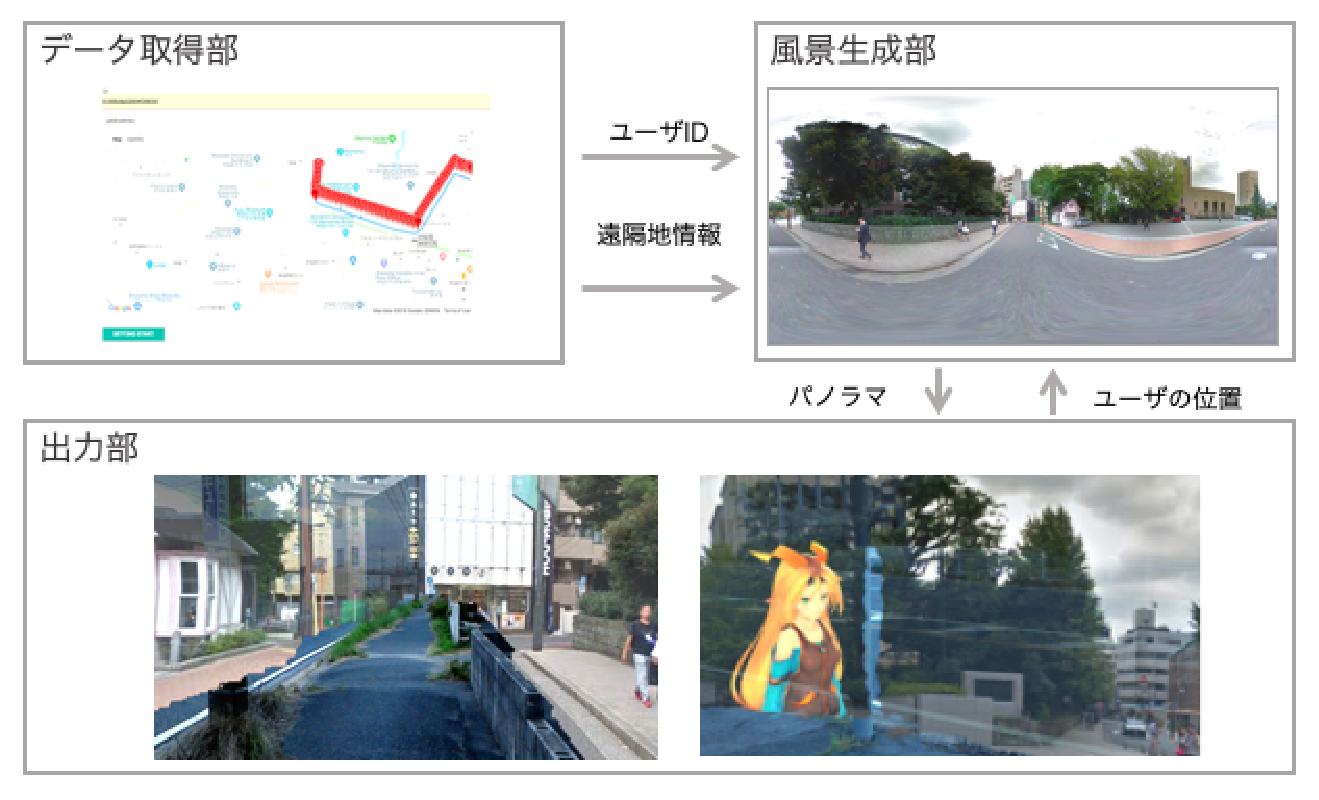
\includegraphics[width=16cm]{img/04_detail/system.eps}
  \caption{本システムの構成}
  \label{figure:system}
 \end{center}
\end{figure}

\clearpage
 
\subsection{システム利用イメージ}
本システムを利用する際,ユーザはまずHololensを装着し,風景表示を行うアプリケーションを起動する.起動した際に表示されるHololensの端末IDを,遠隔旅行を行うコース設定用Webページで入力する.その後Webページに表示されているマップ上をクリックする事で遠隔旅行コースの出発地点,目的地点を設定する.システムは出発地点と目的地点を繋ぐコースが生成し,コース上のパノラマ画像を取得する.パノラマ画像の取得が完了したら,Hololens上で遠隔地の風景が表示され遠隔旅行をする事が可能になる.
図\ref{figure:usecase}は遠隔地としてローマのコロッセオを設定し,遠隔旅行を体験している例である.

\begin{figure}[ht]
 \begin{center}
  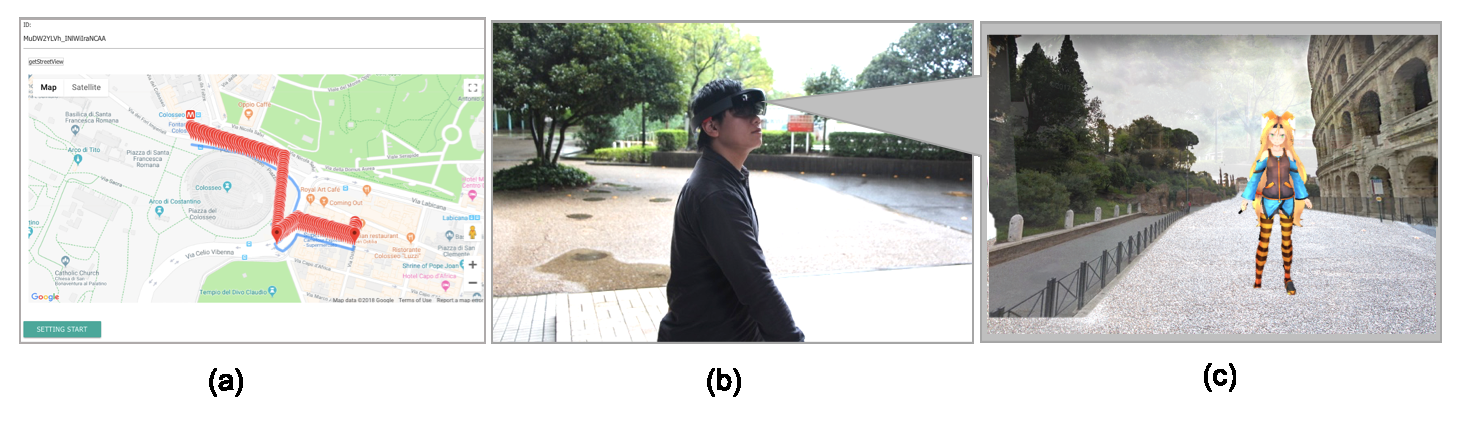
\includegraphics[width=16cm]{img/04_detail/useimage.eps}
  \caption{システム利用イメージ}
  \label{figure:usecase}
 \end{center}
\end{figure}

\clearpage
% データ取得部
\subsection{データ取得部}
データ取得部は,出力部でのユーザ識別,ユーザ毎の風景表示のため,ユーザ情報,遠隔地のStreetViewに関する情報を取得する処理群である.データは遠隔地設定ページでユーザが入力した値を使用する.取得したデータはデータベースに保存し管理する.本システムではUnityの標準クラスで利用可能な軽量データ交換フォーマットJSONを利用しデータを管理する\cite{json}.
以下にJSONに含まれる各データの詳細を示す.

\begin{table}[ht]
  \begin{tabular}{| c | l |}
  \hline
    ユーザID & ユーザを識別するための固有ID \\ \hline
    表示遠隔地 & 遠隔地の情報からユーザが現在見ている遠隔地の場所を抽出するための値\\ \hline
    遠隔地の情報群 & 指定遠隔地の経度,緯度,パノラマID \\ \hline
  \end{tabular}
\end{table}

\clearpage

\subsubsection{ユーザ情報取得}
ユーザ情報取得部ではユーザの識別のために使用する固有のユーザIDを取得する.ユーザIDとしてユーザが使用するHololensの端末IDを使用する. 遠隔旅行をするコースの設定用Webページでユーザが入力したHololensの端末IDをサーバに送信し,データベースを更新する.これによりシステムを使用する際にどのユーザがどのアバターの制御するかを識別する.

\clearpage

\subsubsection{StreetView情報取得部}
コース設定部ではユーザが選択した 2つのポイ ントを出発地と目的地とし, 徒歩での移動コースを 生成する. コースの生成は GoogleMapsApi を用いて行なう\cite{googlemapsapi}. 
生成したコース上にStreetViewを取得する座標を一定の間隔で設定する.Google が定めた StreetView 認定要件において StreetView 間の距離は 3 メートルとなっていたため\cite{svrule}. コース上に設定するStreetViewを取得する座標の間隔は 3 メートルとした. StreetViewを取得する座標の設定方法はまずコース上からカーブや曲がり角を全て抽出し, それぞれの座標を記録する. その後抽出した座標間を 3 メートル間隔で分割し, StreetViewを取得する座標を設定する. 
その後Google Maps APIを用いて3メートル感覚で取得した座標からStreetViewのパノラマ画像が持つ固有のパノラマIDを取得する.取得したパノラマIDと座標をデータベースに書き込み更新をする.データベースへの書き込みは出発地点の座標からはじめ,同じパノラマIDを持つ座標は書き込みを行わないようにした.これによりデータベースでパノラマIDが重複する事を防ぐ.



%図\ref{figure:setcource}は

%図 9 の例ではコース上から 3 つの曲がり角の座標を記録し, 更に各座標間において 3 メートル間隔で StreetView を取得するポイントを計 78 ポイント設定している.



\clearpage

% 風景生成部
\subsection{風景生成部}
風景生成部はデータ取得部で取得したStreetViewの情報からパノラマ画像の生成,道路部分切り抜きを行い,出力部へと送る風景画像を生成する処理群である.
\subsubsection{パノラマ画像生成}
パノラマ画像の生成にはGSVPanoライブラリを利用した\cite{GSVpano}.GSVPanoライブラリはGoogleStreetView からパノラマ画像を作成するライブラリである.パノラマ画像の生成は図\ref{figure:panorama}のようにパノラマ表示されたGoogleStreetViewについて複数の視線の向きで28枚の画像を取得する.その後パノラマ画像になった時,隣接する部分の画像どうしを結合することで一枚のパノラマ画像を生成する.
その後システムは生成したパノラマ画像トリミングすることで余白部分の削除を行う.

\begin{figure*}[ht]
\begin{center}
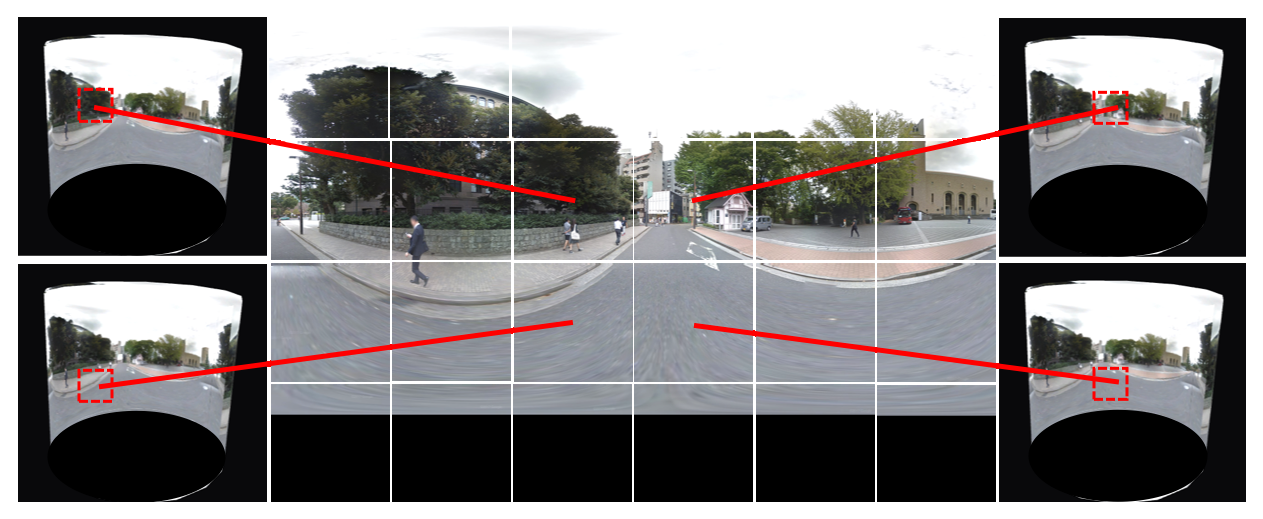
\includegraphics[width=17cm]{img/04_detail/make_panorama.eps}
\end{center}
\caption{パノラマ画像の生成}
\label{figure:panorama}
\end{figure*} 

\clearpage

\subsubsection{道路部分切り抜き}
StreetView 取得部で取得した画像に対し道路部の切り抜きを行う. 切り抜きにはマスク処理を用いる. マスク画像は事前に手動で StreetView の道路部分を黒くし, 風景部分を白くすることで作成した. StreetView取得部で取得した画像に対し図\ref{figure:trim}のようにマスク画像を用いてマスク処理を行い道路部分を切り抜く.


\begin{figure}[h]
\begin{center}
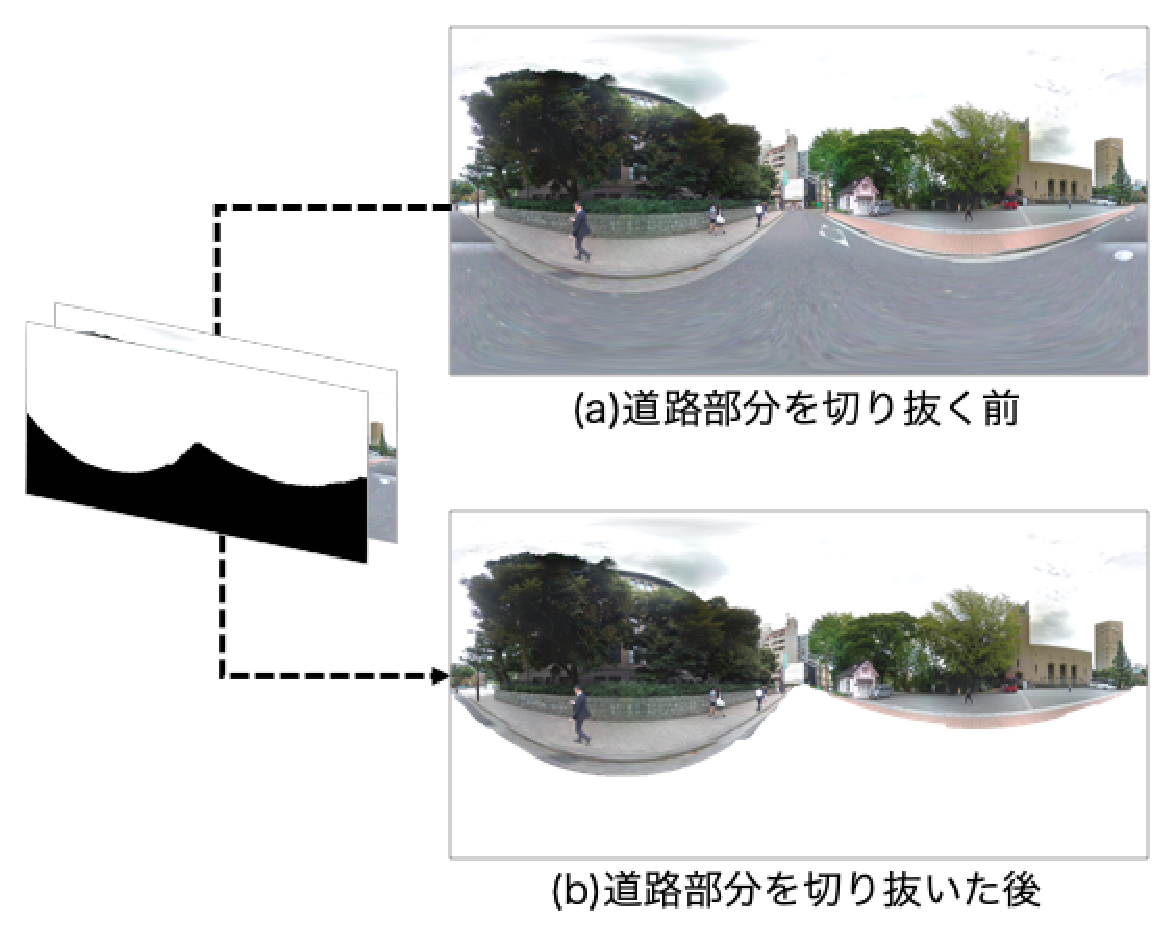
\includegraphics[width=11cm]{img/04_detail/triming.eps} 
\end{center}
\caption{マスク処理による道路部分の切り取り}
\label{figure:trim}
\end{figure} 
%\clearpage
\clearpage
% 出力部
\subsection{出力部}
出力部は風景生成部で生成したパノラマ画像とデータ取得部で取得したユーザ情報を元に風景,他ユーザの表示,またユーザの移動による風景の更新を行う処理群である. ユーザ A とユーザ Bがレクリエーションしている出力例を図\ref{figure:output}に示す.
(a),(b)はそれぞれ ユーザ A, ユーザ Bが実際にいる場所の風景である.(c) はユーザ A, ユーザ Bが遠隔旅行こーすとして設定した場所(東京)の風景を示している.(d)は ユーザ A, ユーザ Bが実際にいる場所と, 指定した遠隔地の位置関係である. (e)はユーザ Aから見える風景である.現実空間に遠隔地が重畳され,同じ遠隔地を指定したユーザ Bのアバターが表示されている.(f)は反対にユーザ Bから見える風景である. (g)はシステム使用時の遠隔地における二人のユーザの位置関係である.

\begin{figure*}[ht]
\begin{center}
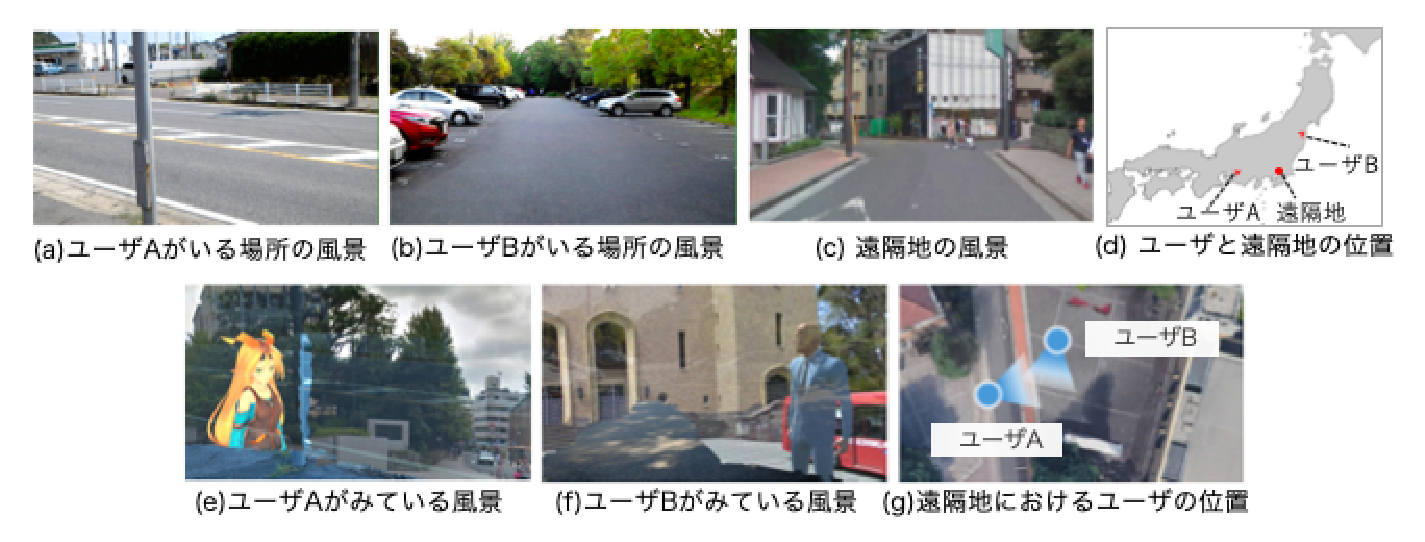
\includegraphics[width=17cm]{img/04_detail/output.eps}
\end{center}
\caption{システム使用例と出力}
\label{figure:output}
\end{figure*} 

\subsubsection{風景表示}
現実風景への重畳は球体のオブジェクトにテクスチャとして風景生成部で生成したパノラマ画像を貼り付けることで行う.
パノラマ画像を貼り付けた球体オブジェクトの内部にシステム起動時ユーザの視点となるUnityのカメラオブジェクトを配置する.
これにより周囲の風景は遠隔地の風景へと変化する.


\clearpage

\subsubsection{他ユーザの表示}
他ユーザの表示ではユーザが表示している遠隔地が近い他ユーザのアバターを表示する.アバターとしてUnityのAsset Storeで無料配布されているUnityちゃんを使用した\cite{unitychan}.
ユーザ間のアバターの同期処理にはオンラインゲームの同期処理に使われる Photon Unity Cloud を利用した\cite{photon}.
表示するユーザはデータ取得部で生成したJSONデータを元に決定する.
システムはJSONデータのユーザ情報と現在地情報から,表示する遠隔地同士の距離が近いユーザのユーザIDを取得する.
そして取得したユーザIDを元にPhoton Unity Cloud のルームを検索する.ユーザは取得した近いユーザのIDと同じ名前のルームが存在する場合,入室する.検索した結果近いユーザのIDと同じ名前のルームがなければシステムは自身のユーザIDと同名のルームを作成する.
これにより他ユーザとのアバターの共有を行う.
アバターの向きはHololensの
$\it{y}$
軸方向のみ同期していおり,図 \ref{figure:abatar}(a)のようにアバターの回転を水平方向のみに制限している.またアバターの座標はHololensの座標と同期しており,図\ref{figure:abatar}(b)のようにユーザが進行した方向に動く.

\begin{figure}[h]
\begin{center}
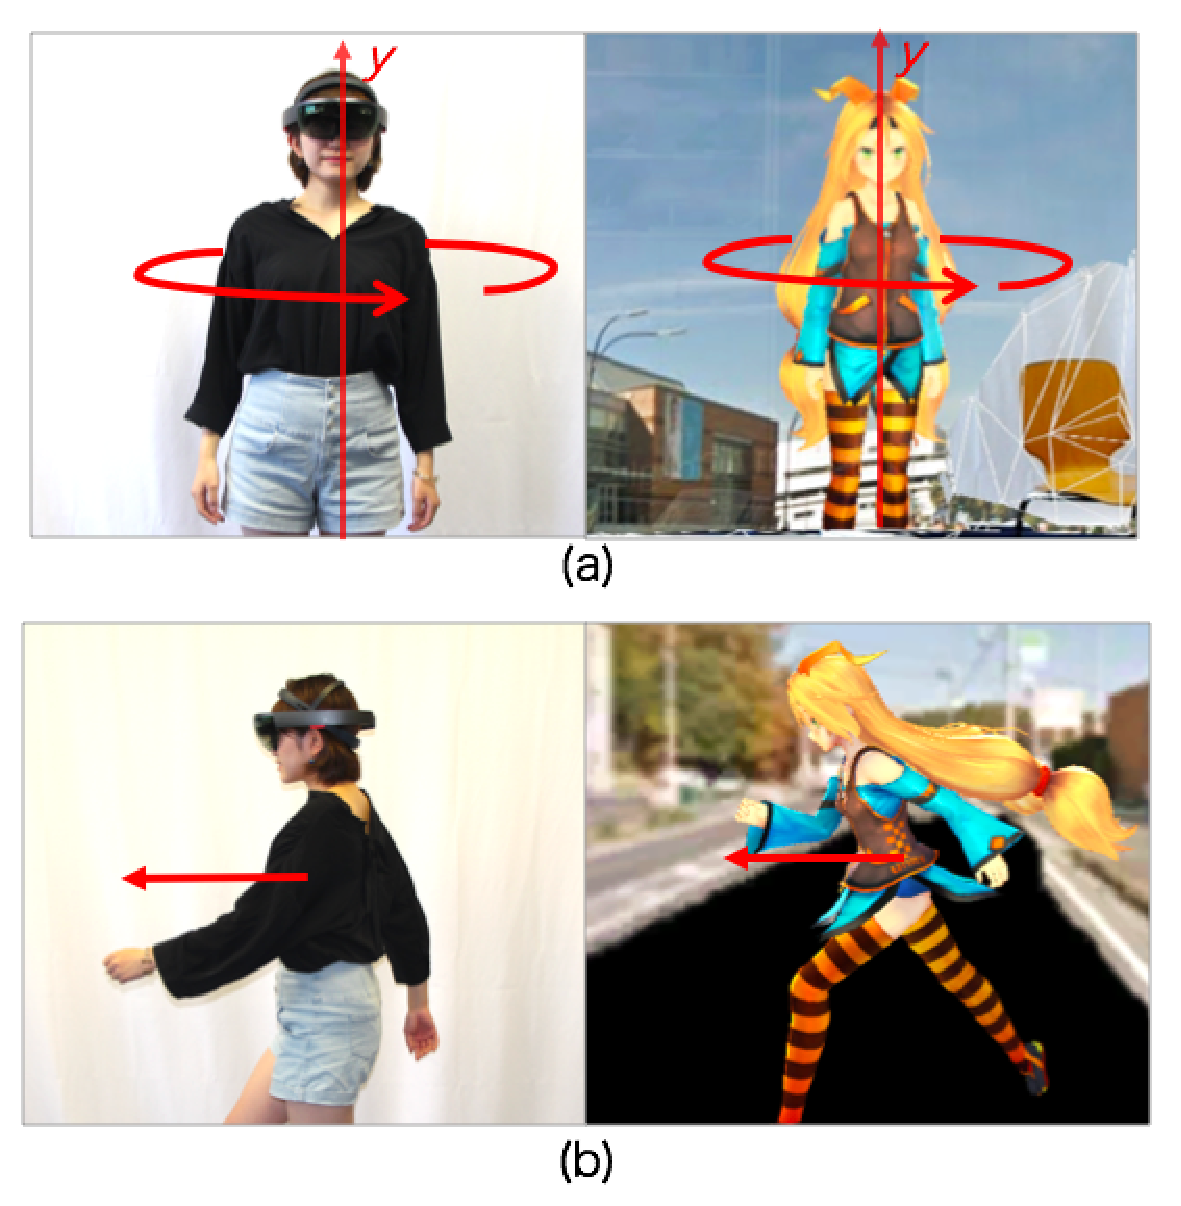
\includegraphics[width=11cm]{img/04_detail/avatar_move.eps} 
\end{center}
\caption{アバターの動き}
\label{figure:abatar}
\end{figure} 

\clearpage

\subsubsection{風景更新}
風景更新ではユーザが歩くことでパノラマ画像を更新する.ユーザの位置はHololens の自己位置推定機能によって算出する.自己位置推定機能とはHololensのアプリケーション起動時の座標との相対距離を推定する機能である. HololensとUnityのカメラオブジェクトは座標と方向が同期されているため,カメラオブジェクトの座標を取得することで自己位置を推定が可能である.風景の更新はHololensが3メートル座標移動するごとに行う.これはGoogle が定めた StreetView 認定要件において StreetView 間の距離が3 メートルとなっていたためである.
システムは風景更新時のHololensの座標と,前回の更新時のHololensの座標から移動方向を算出し,ユーザの移動方向に道が続くように風景表示用の球体オブジェクトを回転させる.
移動方向の算出にはUnityのVector3クラスに定義されている,GetAim関数により算出できる.
%\clearpage
